\documentclass[12pt, a4paper]{article}

\usepackage{import}
\usepackage{standalone}

\usepackage[top=4cm, right=2cm, bottom=2.7cm, left=2cm]{geometry}

\usepackage{wrapfig}
\usepackage{tabulary}
\usepackage{float}
\usepackage{pifont}
\usepackage{background}
\usepackage{tikz}


\pagestyle{empty}
\setlength{\parindent}{0pt}

\begin{document}
	\begin{minipage}{\textwidth}
		\section{Groepswerk \hfill\small Bron: Bebras}
			Grote Bever leert aan vier groepen van jonge bevers hoe ze een dam moeten bouwen. Dit is een heel delicate onderneming. Soms moet \'e\'en bever wachten op enkele van de andere bevers totdat die hun werk hebben afgewerkt vooraleer hij aan het zijne kan beginnen. Grote Bever heeft geluisterd naar wat elke bever voorzien heeft om te doen en heeft de bijbehorende beperkingen in een schema opgetekend met behulp van pijlen: een pijl van X naar Y betekent dat Y moet wachten totdat X klaar is met zijn werk vooraleer hij zelf kan beginnen. \\
			
			\'E\'en van de groepen zal er niet in slagen zijn dam af te werken. Welke groep is dit?
			
			\begin{table}[H]
				\centering
				\begin{tabulary}{\linewidth}{|C|C|}
					\hline
					\textbf{A} \vspace{0.2cm}
					
					
\includegraphics[width=0.9\linewidth]{option1}
					&
					\textbf{B} \vspace{0.2cm}
					
					
\includegraphics[width=0.9\linewidth]{option2}
					\\ \hline
					\textbf{C} \vspace{0.2cm}
					
					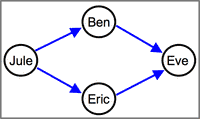
\includegraphics[width=0.9\linewidth]{option3}
					&
					\textbf{D} \vspace{0.2cm}
					
					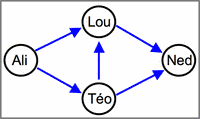
\includegraphics[width=0.9\linewidth]{option4}
					\\ \hline 
				\end{tabulary}
			\end{table}
	\end{minipage} \\ \\
	
\end{document}	